

\subsection{Deformation retraction}

%The algebras we have been developing so far are all well and interesting, but sometimes, we wish to have a little less structure, or ``looser'' structure. This reasoning prompts the study of so-called ``higher algebra''. An $\A$-algebra is one of these higher structures, that arose quite naturally in topology, but have since been given their own algebraic theory. They first showed up when Stasheff was studying loop spaces in his phd thesis. 

%We have already told a bit about the connection between topological spaces and DG-algebras, so it should not come as a surprise when these $\A$ structures also show up in our more algebraic setting. It turns out that being a DG-algebra is not a stable property under homotopy. More specifically, given a DG-algebra $A$, a chain complex $B$, and a deformation retract of $A$ onto $B$, then we cant induce a DG-algebra structure on $B$. But, if we try, the induced structure will instead be an $\A$ structure. Lets make this a bit more precise. 

Let's try to apply the above topological motivation to our more algebraic situation. As DG-algebras are in particular cochain complexes, we can ask weather being a DG-algebra is a stable property under homotopy equivalences in $Ch(Vect_k)$, the category of cochain complexes of vector spaces. What we mean by this is that given a DG-algebra $A$, and a cochain complex $V$ that is homotopy equivalent to $A$, can we induce a DG-algebra structure onto $V$? This will in some sense tell us weather the homotopy theory of DG-algebras is well behaved. To make things even more simple, we use deformation retractions instead of homotopy equivalences. 

\begin{definition}[Deformation retraction]
\label{def:deformation_retraction}
Let $(A, d_A)$ and $(B, d_B)$ be cochain complexes, and let $p:A\longrightarrow B$ and $i:B\longrightarrow A$ be morphisms between them. We call $p$ a deformation retraction if $p\circ i = id_B$ and there exists a homotopy $i\circ p\overset{h}\sim id_A$. If there exists a deformation retraction $A\longrightarrow B$, then we say $B$ is a deformation retract of $A$, or that $A$ deformation retracts onto $B$.

We sometimes denote such a system by $(A, B, p, i, h)$, and more often with the following diagram:
\begin{center}
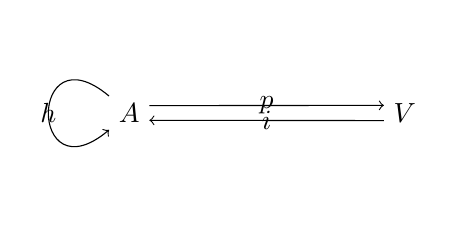
\begin{tikzpicture}
	\node (1) {$A$};
	\node (2) [node distance=3.5cm, right of=1] {$V$};
	
	\draw [to-, out=220, in=140, loop] (1) to node {$h$} (1);
	\draw [-to] (1.20) to node {$p$} (2.160);
	\draw [-to] (2.200) to node {$i$} (1.340);
\end{tikzpicture}
\end{center}
\end{definition}

Note that a deformation retraction is in particular a homotopy equivalence. In fact, two cochain complexes are homotopy equivalent if and only if they are both deformation retracts of another cochain complex. Hence these deformation retracts are intimately linked with the homotopy theory of cochain complexes. A DG-algebra is in particular a cochain complex, so it is then perhaps natural to ask weather two homotopy equivalent complexes are DG-algebras if and only if the other one is, or equivalently, is the deformation retract of a DG-algebra again a DG-algebra? As stated earlier this is not the case. 

In order to get correct signs when working with graded objects we will use the \emph{Koszul sign rule}\index{Koszul sign rule} a lot. This tells us how to get signs when applying tensor products of functions to tensors, as well as composing tensor products of functions. These rules are as follows: 
\begin{equation*}
    (f\otimes g)(a\otimes b) = (-1)^{|a||g|}f(a)\otimes g(b)
\end{equation*} 
for applying functions to tensors, and
\begin{equation*}
    (f_1\otimes g_1)\circ (f_2\otimes g_2) = (-1)^{|f_2||g_1|}f_1\circ f_2 \otimes g_1\circ g_2
\end{equation*}
for composition of functions. All the above, and all future tensors are over $k$. 

Ok, let's now consider the deformation retract
\begin{center}
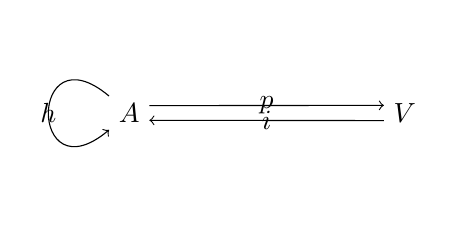
\begin{tikzpicture}
	\node (1) {$A$};
	\node (2) [node distance=3.5cm, right of=1] {$V$};
	
	\draw [to-, out=220, in=140, loop] (1) to node {$h$} (1);
	\draw [-to] (1.20) to node {$p$} (2.160);
	\draw [-to] (2.200) to node {$i$} (1.340);
\end{tikzpicture}
\end{center}

If we try to do the same as we did for the topological case in the motivation, we get an attempted multiplication $m_2 = p\circ m \circ (i\otimes i)$. If we investigate the properties of this product a bit, we notice that it is not associative by the exact same reason given earlier. As before we get two different non-equivalent ways of combining the product with it self:
\begin{itemize}
    \item $m_2(m_2\otimes id)$
    \item $m_2(id\otimes m_2)$
\end{itemize}
We know they are not equal, so what is the next best thing we could hope for? It is of course a homotopy between them. In the motivation we just claimed that there is such a homotopy, but now we want to be very explicit, and very thorough by proving that this is in fact the case. We do this because it will be important as an intuition for the $\A$-algebras we want to construct in the next section. 

Notice that $m_2(m_2\otimes id)$ and $m_2(id\otimes m_2)$ are elements of $Hom(A^{\otimes 3}, A)$ and are both maps of degree zero. Let's draw them in a diagram
\begin{center}
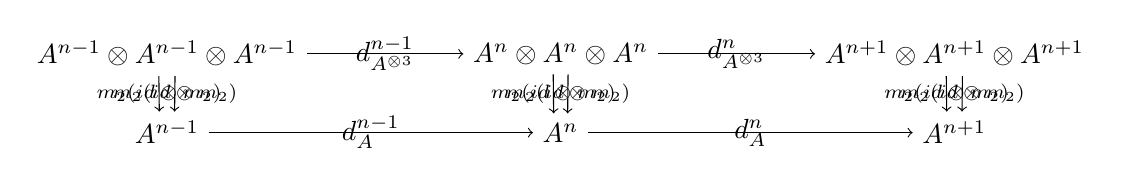
\begin{tikzpicture}
	\node (1) {$A^{n-1}\otimes A^{n-1}\otimes A^{n-1}$};
	\node (2) [node distance=5cm, right of=1] {$A^n\otimes A^n\otimes A^n$};
	\node (3) [node distance=5cm, right of=2] {$A^{n+1}\otimes A^{n+1}\otimes A^{n+1}$};
	
	\node (4) [below of=1] {$A^{n-1}$};
	\node (5) [node distance=5cm, right of=4] {$A^n$};
	\node (6) [node distance=5cm, right of=5] {$A^{n+1}$};

	\draw [-to] (1.250) to node [swap]{{\scriptsize $m_2(id\otimes m_2)$}} (4.110);
	\draw [-to] (1.290) to node {{\scriptsize $m_2(id\otimes m_2)$}} (4.70);
	\draw [-to] (2.250) to node [swap]{{\scriptsize $m_2(id\otimes m_2)$}} (5.110);
	\draw [-to] (2.290) to node {{\scriptsize $m_2(id\otimes m_2)$}} (5.70);
	\draw [-to] (3.250) to node [swap]{{\scriptsize $m_2(id\otimes m_2)$}} (6.110);
	\draw [-to] (3.290) to node {{\scriptsize $m_2(id\otimes m_2)$}} (6.70);
	\draw [-to] (1) to node {$d^{n-1}_{A^{\otimes 3}}$} (2);
	\draw [-to] (2) to node {$d^{n}_{A^{\otimes 3}}$} (3);
	\draw [-to] (4) to node [swap]{$d^{n-1}_{A}$} (5);
	\draw [-to] (5) to node [swap]{$d^{n}_{A}$} (6);
\end{tikzpicture}
\end{center}

This space, $Hom(A^{\otimes 3}, A)$, can be made into a chain complex by defining a boundary operator. If $f$ is just some generic element in $Hom(A^{\otimes 3}, A)$ of degree $|f|$, we define such an operator by
\begin{equation*}
    \partial f = d_A f - (-1)^{|f|} f d_{A^{\otimes 3}}
\end{equation*}
where $d_{A^{\otimes 3}} = (d_A, id, id)+(id, d_A, id)+(id, id, d_A)$. 

A homotopy between $m_2(id\otimes m_2)$ and $m_2(m_2\otimes id)$ would be a map $h\colon A^{\otimes 3}\longrightarrow A$ of degree $-1$, such that $d_A^{n-1}\circ h^{n} + h^{n+1}\circ d_{A^{\otimes 3}}^n = m_2(id\otimes m_2)-m_2(m_2\otimes m_2)$. In or diagram it would be a diagonal map
\begin{center}
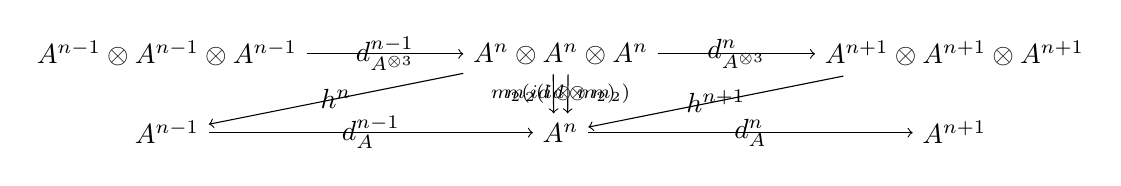
\begin{tikzpicture}
	\node (1) {$A^{n-1}\otimes A^{n-1}\otimes A^{n-1}$};
	\node (2) [node distance=5cm, right of=1] {$A^n\otimes A^n\otimes A^n$};
	\node (3) [node distance=5cm, right of=2] {$A^{n+1}\otimes A^{n+1}\otimes A^{n+1}$};
	
	\node (4) [below of=1] {$A^{n-1}$};
	\node (5) [node distance=5cm, right of=4] {$A^n$};
	\node (6) [node distance=5cm, right of=5] {$A^{n+1}$};

	\draw [-to] (2) to node [swap]{$h^n$} (4);
	\draw [-to] (3) to node {$h^{n+1}$} (5);
	\draw [-to] (2.250) to node [swap]{{\scriptsize $m_2(id\otimes m_2)$}} (5.110);
	\draw [-to] (2.290) to node {{\scriptsize $m_2(id\otimes m_2)$}} (5.70);
	\draw [-to] (1) to node {$d^{n-1}_{A^{\otimes 3}}$} (2);
	\draw [-to] (2) to node {$d^{n}_{A^{\otimes 3}}$} (3);
	\draw [-to] (4) to node [swap]{$d^{n-1}_{A}$} (5);
	\draw [-to] (5) to node [swap]{$d^{n}_{A}$} (6);
\end{tikzpicture}
\end{center}
such that the sum of the outer parallelogram equals the difference of the vertical arrows. But, notice that this is exactly just showing that $\partial h = m_2(id\otimes m_2)-m_2(m_2\otimes id)$!

The explicit homotopy that we will use is the following tertiary operator $m_3$ on $V$
\begin{equation*}
    m_3 = p\circ (m(hm\otimes id)-m(id\otimes hm))\circ (i\otimes i \otimes i),
\end{equation*}
where $m$ denotes the product in $A$. Notice that we have $|m_3|=-1$, and $\partial m_3 = dm_3 + m_3 d_{A^{\otimes 3}}$. Hence for $m_3$ to be the homotopy we want between $m_2(id\otimes m_2)$ and $m_2(m_2\otimes id)$ we must show that $\partial m_3 = m_2(id\otimes m_2)-m_2(m_2\otimes id)$. As we have not come upon a fully written out detailed proof, we have included it to have at least one existing complete calculation in the world. It is not pretty, and it is just tedious straight forward calculation, but in our opinion it is nice to have, as it gives some insight into how these homotopies between operations work. 

We denote $d_A$ by just $d$, and $id$ by $1$ in order to make it more distinguishable from $d$ and eventual copies of $i\circ d$. We also skip writing $\circ$, and denote it instead just by concatenation, so $d\circ m_3 = dm_3$. Since $m_3$ consists of $i, p$, which are both of degree $0$, and $h$, which has degree $-1$, we have $|m_3|=-1$. The boundary of $m_3$ is then
\begin{align*}
    \partial m_3 
    &= dm_3+m_3(d,1,1)+m_3(1,d,1)+m_3(1,1,d)\\
    &= dm_3
    +p((-1)^{|1||d|}m(hm(id\otimes i)\otimes i)
    -(-1)^{|hm||d|}m(id\otimes hm(i\otimes i))) \\
    & \hspace{13mm} 
    +p((-1)^{|1||1|}m(hm(i\otimes id)\otimes i)
    -(-1)^{|hm||1|}m(i\otimes hm(id\otimes i))) \\
    & \hspace{13mm} 
    +p((-1)^{|1||1|}m(hm(i\otimes i)\otimes id)
    -(-1)^{|hm||1|}m(i\otimes hm(i\otimes id)))
\end{align*}

where the signs appear due to the Koszul grading rule. As the identity morphism has degree $0$ most of these vanish, except for $(-1)^{|hm||d|}$. The composite map $hm$ has degree $|h|+|m| = -1+0 = -1$ and the differential $d$ has degree $1$ as we work with cohomological grading. Since $i$ is a morphism of chain complexes it commutes with the differentials, hence we can put all the $i$'s to the right, to get 
\begin{align*}
    \partial m_3 
    &= dm_3
    +p(m(hm(d\otimes 1)\otimes 1)
    +m(d\otimes hm) \\
    & \hspace{17mm} 
    +m(hm(1\otimes d)\otimes 1)
    -m(1\otimes hm(d\otimes 1)) \\
    & \hspace{17mm} 
    +m(hm\otimes d)
    -m(1\otimes hm(1\otimes d))(i\otimes i\otimes i)
\end{align*}

We haven't touched the $dm_3$ part yet, so lets see what this gives us. We get 
\begin{align*}
    dm_3 
    &= 
    d(p(m(hm\otimes 1)
    -m(1\otimes hm))(i\otimes i\otimes i)) \\
    &= 
    p(dm(hm\otimes 1)
    -dm(1\otimes hm))(i\otimes i\otimes i) \\
\end{align*}

Since $A$ is a DG-algebra we can use the graded Leibniz rule to expand $dm$ into $m(d\otimes 1)+m(1\otimes d)$. Doing so both places they appear above gives us
\begin{align*}
    dm_3 
    &= 
    p((m(d\otimes 1)
    +m(1\otimes d))(hm\otimes 1) \\
    &\quad 
    -(m(d\otimes 1)
    +m(1\otimes d))(1\otimes hm))(i\otimes i\otimes i) \\
    &=
    p((m(d\otimes 1)
    +m(1\otimes d))(hm\otimes 1) \\
    &\quad 
    -m(d\otimes 1)
    -m(1\otimes d)(1\otimes hm))(i\otimes i\otimes i) 
\end{align*}

To contract this we again need to apply the Koszul grading rule. For the individual pieces in the above equation we get
\begin{align*}
    m(d\otimes 1)(hm\otimes 1) &= (-1)^{|1||hm|}m(dhm\otimes 1) \\
    m(1\otimes d)(hm\otimes 1) &= (-1)^{|d||hm|}m(hm\otimes d) \\
    m(d\otimes 1)(1\otimes hm) &= (-1)^{|1||1|}m(d\otimes hm) \\
    m(1\otimes d)(1\otimes hm) &= (-1)^{|d||1|}m(1\otimes dhm),
\end{align*}

where as before all signs are $1$ except $(-1)^{|d||hm|}=-1$. Hence we have 
\begin{align*}
    dm_3 
    &= 
    p(m(dhm\otimes 1)-m(hm\otimes d)-m(d\otimes hm)-m(1\otimes dhm))(i\otimes i\otimes i)
\end{align*}

We know that $h$ is a homotopy between $i\circ p$ and $id_A$, and for chain complexes this means that $dh+hd=i\circ p - id_A$. This gives us that we can replace $dh$ by $id_A-i\circ p-hd$ in the equation above. Doing this gives us 
\begin{align*}
    dm_3 
    &= 
    p(m((1-ip-hd)m\otimes 1)-m(hm\otimes d)-m(d\otimes hm) \\
    &\quad -m(1\otimes (1-ip-hd)m))(i\otimes i\otimes i) \\
    &= 
    p(m(m\otimes 1)-m(ipm\otimes 1)-m(hdm\otimes 1) \\
    &\quad -m(hm\otimes d)-m(d\otimes hm) \\
    &\quad -m(1\otimes m)+m(1\otimes ipm)+m(1\otimes hdm))(i\otimes i\otimes i)
\end{align*}

Notice that we have both $m(m\otimes 1)$ and $m(1\otimes m)$ present, with the opposite signs. These two are just repeated products in $A$, so their difference is $0$, as we know $A$ is a DG-algebra, which in particular have an associative product.

After canceling the associator in $A$, and rearranging the terms a bit nicer, we can venture further by again applying the graded Leibniz rule to the $dm$'s. This gives us
\begin{align*}
    dm_3 
    &=
    p(m(1\otimes ipm)-m(ipm\otimes 1) \\
    &\quad -m(h(m(d\otimes 1)+m(1\otimes d))\otimes 1) \\
    &\quad -m(hm\otimes d)-m(d\otimes hm) \\
    &\quad +m(1\otimes h(m(d\otimes 1)+m(1\otimes d))))(i\otimes i\otimes i) \\
    &=
    p(m(1\otimes ipm)-m(ipm\otimes 1) \\
    &\quad - m(hm(d\otimes 1)\otimes 1) - m(hm(1\otimes d)\otimes 1) \\
    &\quad +m(hm\otimes d)+m(d\otimes hm) \\
    &\quad +m(1\otimes hm(d\otimes 1))+m(1\otimes hm(1\otimes d)))(i\otimes i\otimes i)
\end{align*}

Now we are finally ready to put everything together. Recall we wanted to find $\partial m_3 = dm_3 + m_3d_{A^{\otimes 3}}$. The calculation has been so long that it is hard to remember what we actually were doing. We have found both parts of this equation, so putting them together and moving all the $p$'s to the left, and the $i$'s to the right, we get
\begin{align*}
    \partial m_3
    &=
%    p(m(1\otimes ipm)-m(ipm\otimes 1) \\
%    &\quad - m(hm(d\otimes 1)\otimes 1) - m(hm(1\otimes d)\otimes 1) \\
%    &\quad -m(hm\otimes d)-m(d\otimes hm) \\
%    &\quad +m(1\otimes hm(d\otimes 1))+m(1\otimes hm(1\otimes d))(i\otimes i\otimes i) \\
%    &\quad
%    +p(m(hm(d\otimes 1)\otimes 1)
%    +m(d\otimes hm) \\
%    &\quad 
%    +m(hm(1\otimes d)\otimes 1)
%    -m(1\otimes hm(d\otimes 1)) \\
%    &\quad  
%    +m(hm\otimes d)
%    -m(1\otimes hm(1\otimes d))(i\otimes i\otimes i) \\
%    &= 
    p(m(1\otimes ipm)-m(ipm\otimes 1) \\
    &\quad - m(hm(d\otimes 1)\otimes 1) - m(hm(1\otimes d)\otimes 1) \\
    &\quad -m(hm\otimes d)-m(d\otimes hm) \\
    &\quad +m(1\otimes hm(d\otimes 1))+m(1\otimes hm(1\otimes d) \\
    &\quad
    +m(hm(d\otimes 1)\otimes 1)
    +m(d\otimes hm) \\
    &\quad 
    +m(hm(1\otimes d)\otimes 1)
    -m(1\otimes hm(d\otimes 1)) \\
    &\quad  
    +m(hm\otimes d)
    -m(1\otimes hm(1\otimes d))(i\otimes i\otimes i)
\end{align*}
%where in the last equality we have just put the $p$ on the left and the $i$'s on the right. This is just to have everything inside the same bracket, i.e. $p(\text{all the stuff})(i\otimes i\otimes i)$, which we can do as they are linear. 
We see that almost everything on the inside cancels nicely, and we are left with 
\begin{equation*}
    \partial m_3 = p(m(1\otimes ipm)-m(ipm\otimes 1))(i\otimes i\otimes i)
\end{equation*}

Expanding this we get 
\begin{equation*}
    \partial m_3 = pm(1\otimes ipm)(i\otimes i\otimes i) - pm(ipm\otimes 1)(i\otimes i\otimes i)
\end{equation*}

which we recognize as $m_2(1\otimes m_2) - m_2(m_2\otimes 1)$. This means we are finally left with what we wanted to show 
\begin{equation*}
    \partial m_3 = m_2(1\otimes m_2)-m_2(m_2\otimes 1)
\end{equation*}
i.e. the associator of $m_2$. 

Hence we see that the topology we described earlier---with the Stasheff associahedra---really dictates what is going on in the purely algebraic scenario. This is of course by design, as Stasheff used these algebraic structures to describe what happens topologically, but it is still important to understand how the two different stories are compatible. This really shows that $m_3$ is the algebraic version of $K3$, i.e. the interval---or homotopy really---between the two ways of combining the product $m_2$ with it self. Because of this we often call $m_3$ \emph{the associating homotopy}\index{The associating homotopy} of $m_2$. 

Let's test our understanding of this by looking a bit at what happens in the arity four case as well. We have now done the bulk terse computation, so it will luckily not be as difficult, and we will not be as detailed. First let's look at $K4$, with its corresponding ways to combine $m_2$. 

\hspace{2mm}

\begin{center}
\def\svgwidth{0.7\textwidth}
\input{images/K4_operations.pdf_tex}
\end{center}

\hspace{1mm}

We see that we have two paths from $m_2(m_2(m_2\otimes 1)\otimes 1)$ to $m_2(1\otimes m_2(1\otimes m_2))$. We can describe these path explicitly by using the homotopies between the vertices. 

\hspace{1mm}

\begin{center}
\def\svgwidth{0.7\textwidth}
\input{images/K4_homotopies.pdf_tex}
\end{center}

\hspace{1mm}

which makes the two paths equal to
\begin{equation*}
    m_3(m_2\otimes 1\otimes 1) + m_3(1\otimes 1\otimes m_2)
\end{equation*}
and 
\begin{equation*}
    m_2(m_3\otimes m_1)+m_3(1\otimes m_2\otimes 1)+m_2(1\otimes m_3)
\end{equation*}
Without now defining some quaternary operation $m_4$ concretely---we will do this a bit later---we know what its boundary, $\partial m_4$, must look like. It must look like the boundary of $K4$ as a topological space, i.e. 
\begin{equation*}
    \partial m_4 = m_2(1\otimes m_3) - m_3(1\otimes 1\otimes m_2) - m_3(m_2\otimes 1\otimes 1) + m_2(m_3\otimes m_1)+m_3(1\otimes m_2\otimes 1)
\end{equation*}

which we see is the difference of the two paths just described above. Thus, $m_4$ is a homotopy between the two paths. 

We will later look a little bit into what happens for higher arity maps, but things unfortunately get exponentially more complicated. We will then also use a very specific deformation retraction from a DG-algebra onto its cohomology algebra $H(A)$, and use that to equip $H(A)$ with $m_3$ and other higher arity maps which will sort of model the Massey products we saw earlier.  
